
\section{Benchmark tests: ring.erl}
I have run two benchmark test to see how and if the performance is increasing by using one core or more by using the argument \texttt{erl -smp enable} and \texttt{erl -smp disable}. My system is a MacBookAir with a 1,8 GHz Intel Core i7 CPU, so in the enabled mode 4 cores where used. \\
\\
The runtime of the \textit{parallel} executed test took basically more time, so the speedup is in general less the 1 (a deterioration). This could be that the overhead to schedule and manage is bigger than the benefit of parallelisation. But on the other hand in my opinion it is not a good example to parallelise because every process has to wait for the previous process to finish and then the next process can start to process. This is called data dependency and this is very high. \\
\\
In Figure~\ref{fig:example3} the two lines are describing the $\sum = N * M$ and $N$ is the number of processes and $\sum$ is here a constant value $8292$. In this graph you can see that  the performance is decreasing by an increasing number of processes in the case using the argument \texttt{erl -smp enable} when it comes to a number of 512 processes or nodes in the ring. \\
\\
I had a look on the use of the available cores but I have observe that more or less just two CPU where used and the total use was around 100 percent. So I would assume that two cores have alternate to do that task.
\begin{figure}[h!]
	\center
	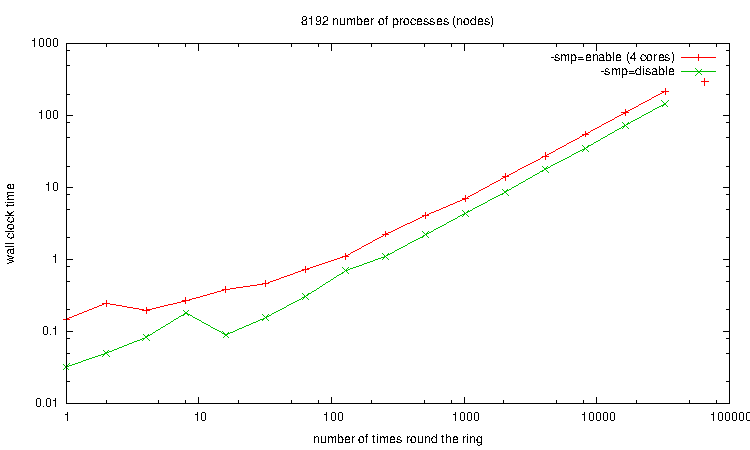
\includegraphics[width=1\textwidth]{img/8192_number_of_processes.pdf}
	\caption{Wall Clock Time by a fixed number of processes and increasing number of rounds in the ring}
    \label{fig:example1}
\end{figure}
\begin{figure}[h!]
	\center
	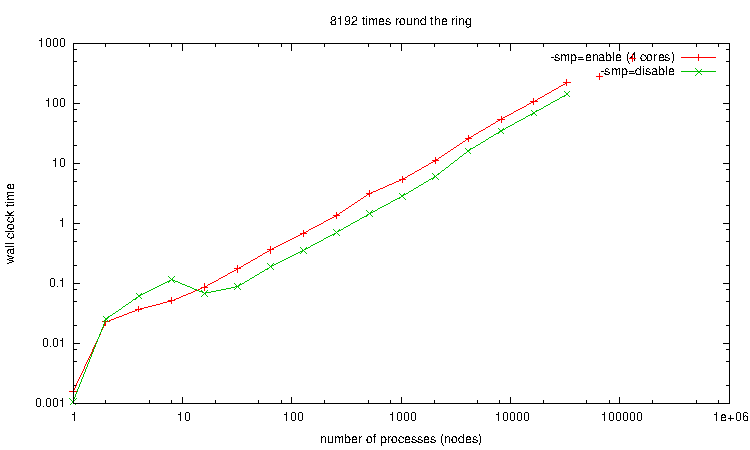
\includegraphics[width=1\textwidth]{img/8192_times_round_the_ring.pdf}
	\caption{Wall Clock Time by a fixed number of rounds and increasing number of processes}
    \label{fig:example2}
\end{figure}

\begin{figure}[h!]
	\center
	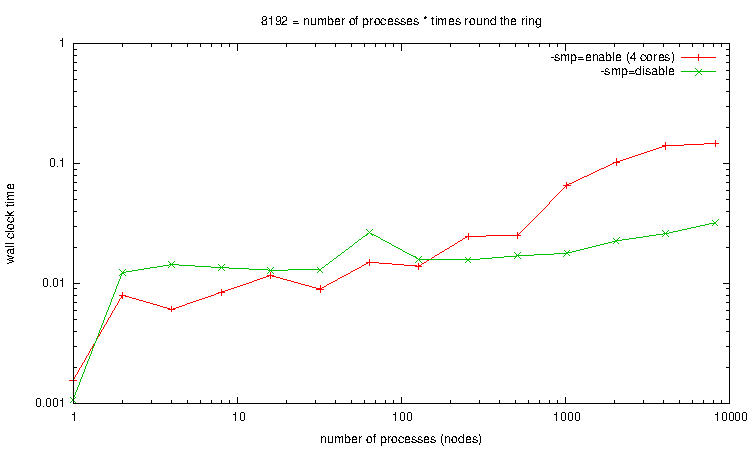
\includegraphics[width=1\textwidth]{img/8192_IS_number_x_times.pdf}
	\caption{Wall Clock Time by increasing number of processes and doing \textit{calculations} to get the sum of 8192.}
    \label{fig:example3}
\end{figure}

% \bibliographystyle{plain}
% \bibliography{literature}

